\chapter{Applicability to Amputee Data}
\label{chp:amputee-data}
% Introduction to chapter
% The first job of the introduction is to tell the reader what your topic is and why it’s interesting or important. This is generally accomplished with a strong opening hook. The hook is a striking opening sentence that clearly conveys the relevance of your topic. Think of an interesting fact or statistic, a strong statement, a question, or a brief anecdote that will get the reader wondering about your topic.
Introduction

% Background - link back to the original research question of the thesis. Can ml methods be used to improve locomotion mode recognition
% Relevant background on the topic - For a paper describing original research, you’ll instead provide an overview of the most relevant research that has already been conducted. This is a sort of miniature literature review—a sketch of the current state of research into your topic, boiled down to a few sentences.
How have other people fared trying to classify amputees? What methods have they used?

% Establish your research problem
% In an empirical research paper, try to lead into the problem on the basis of your discussion of the literature. Think in terms of these questions:
% What research gap is your work intended to fill?
% What limitations in previous work does it address?
% What contribution to knowledge does it make?
Difficult to get data for an amputee - they are less able to walk around require supervision

Use of non-amputee data transfer learning to improve performance of \acrshort{lmr} classifier for an amputee.

% Research question
% Present your research question clearly and directly, with a minimum of discussion at this point. The rest of the paper will be taken up with discussing and investigating this question; here you just need to express it.
% What are the aims of this chapter
% - Present differences between amputee and non-amputee gait
% - Attempt to apply developed techniques to amputee data
% - Identify challenges in adapting techniques developed to amputee data
Can non-amputee data be used to improve the performance/reduce data requirements of a classifier for an amputee

% Sometimes an overview of the chapter
First present the amputee data that has been collected. Then present the results of implementing the personalisation methods. Then discuss the work and it's limitations

%-----------------------------------------------------------------
\section{Amputee Gait Data}
What data have we managed to get? Amputee are using Echelon VT

How is it different from a non-amputee

% Present summaries of amputee gait
Figure \ref{fig:ch6_amputee_gyro_trends} shows the angular velocity of the ankle in the Saggital plane for the intact and prosthetic limbs of a trans-tibial amputee. For reference the same signals are shown for a non-amputee.
% How does it differ from non-amputee gait data
\begin{figure}[p]
    \begin{tabular}{lccc}
        & \textbf{Non-Amputee} & \textbf{Amputee -- Intact Limb} & \textbf{Amputee -- Prosthetic} \vspace{0.2cm}\\

        \rotatebox{90}{\enspace\qquad \textbf{Walking}} &
        \begin{subfigure}[b]{0.275\textwidth}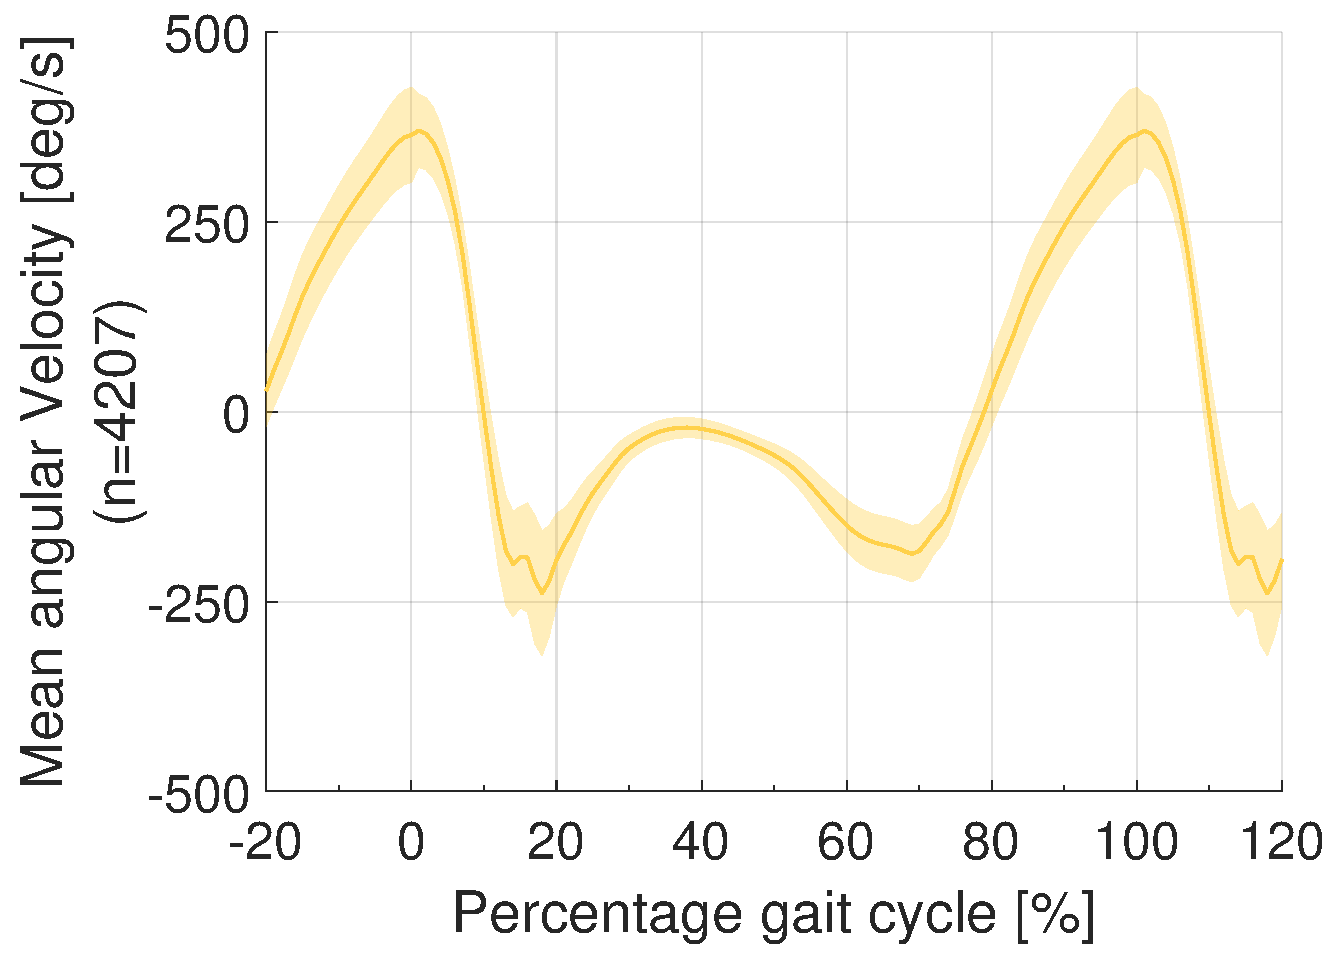
\includegraphics[width=\linewidth]{content/6-Amputee/Gait-Trends/ch6_subject_01_gait_trends_r_ankle_gyro_z_activity_walking.pdf}\end{subfigure} & \begin{subfigure}[b]{0.275\textwidth}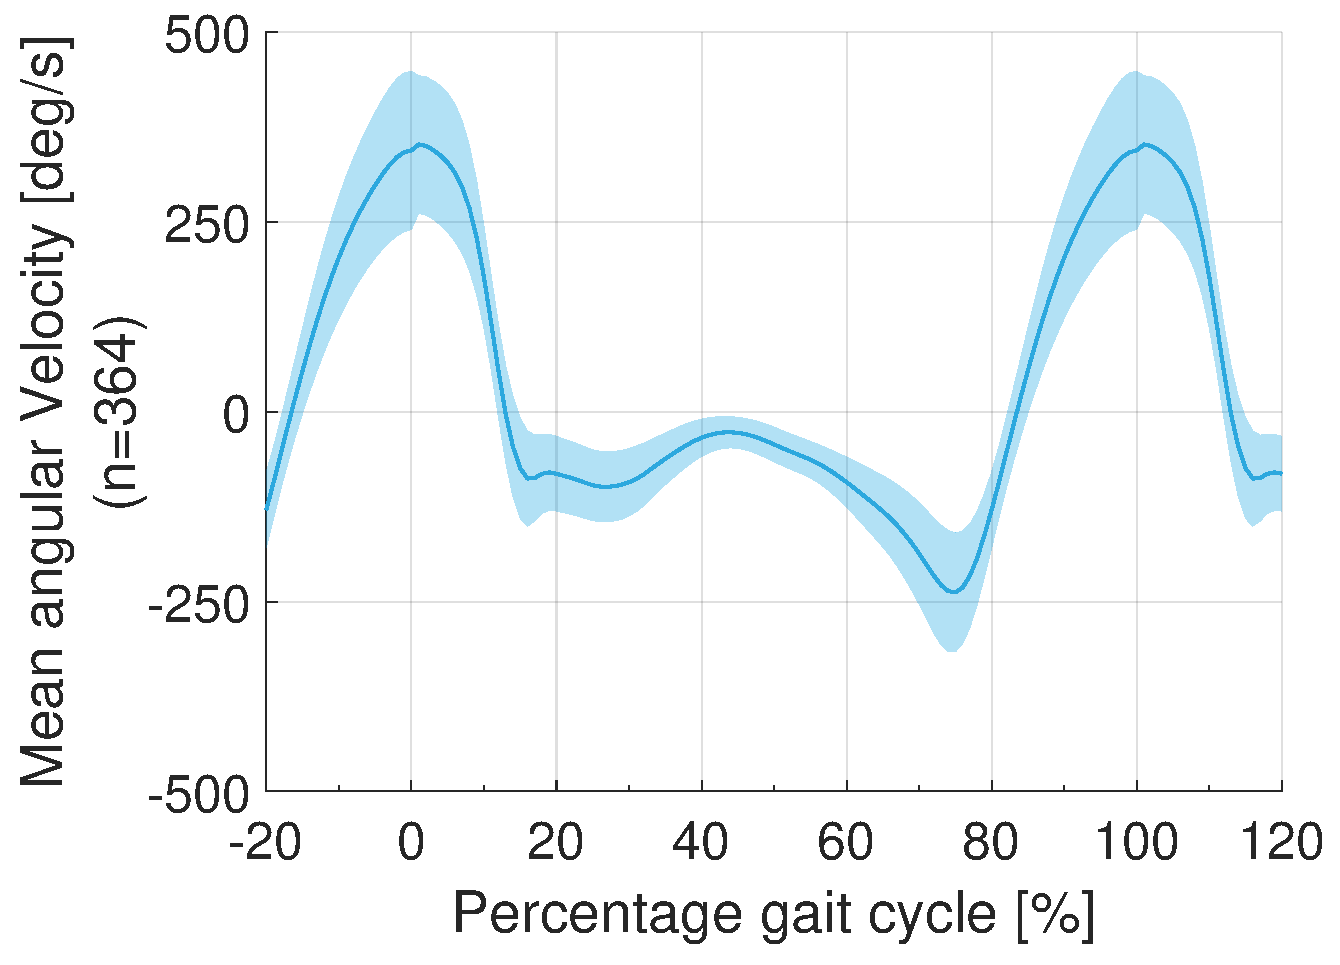
\includegraphics[width=\linewidth]{content/6-Amputee/Gait-Trends/ch6_amputee_gait_trends_l_ankle_gyro_z_activity_walking.pdf}\end{subfigure} &
        \begin{subfigure}[b]{0.275\textwidth}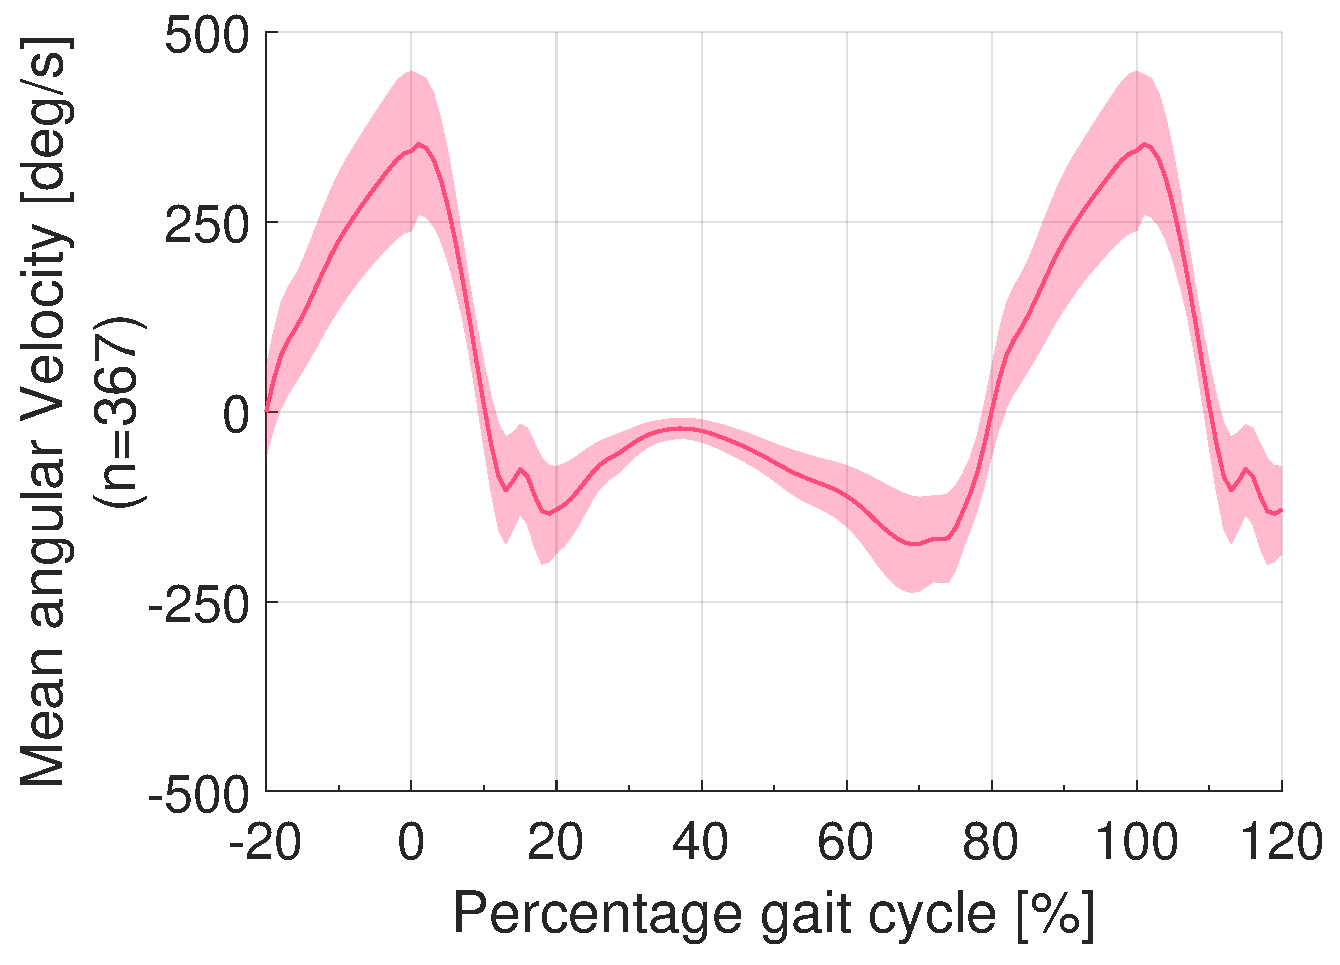
\includegraphics[width=\linewidth]{content/6-Amputee/Gait-Trends/ch6_amputee_gait_trends_r_ankle_gyro_z_activity_walking.pdf}\end{subfigure} \\
        
        \rotatebox{90}{~\quad \textbf{Ramp Ascent}} & 
        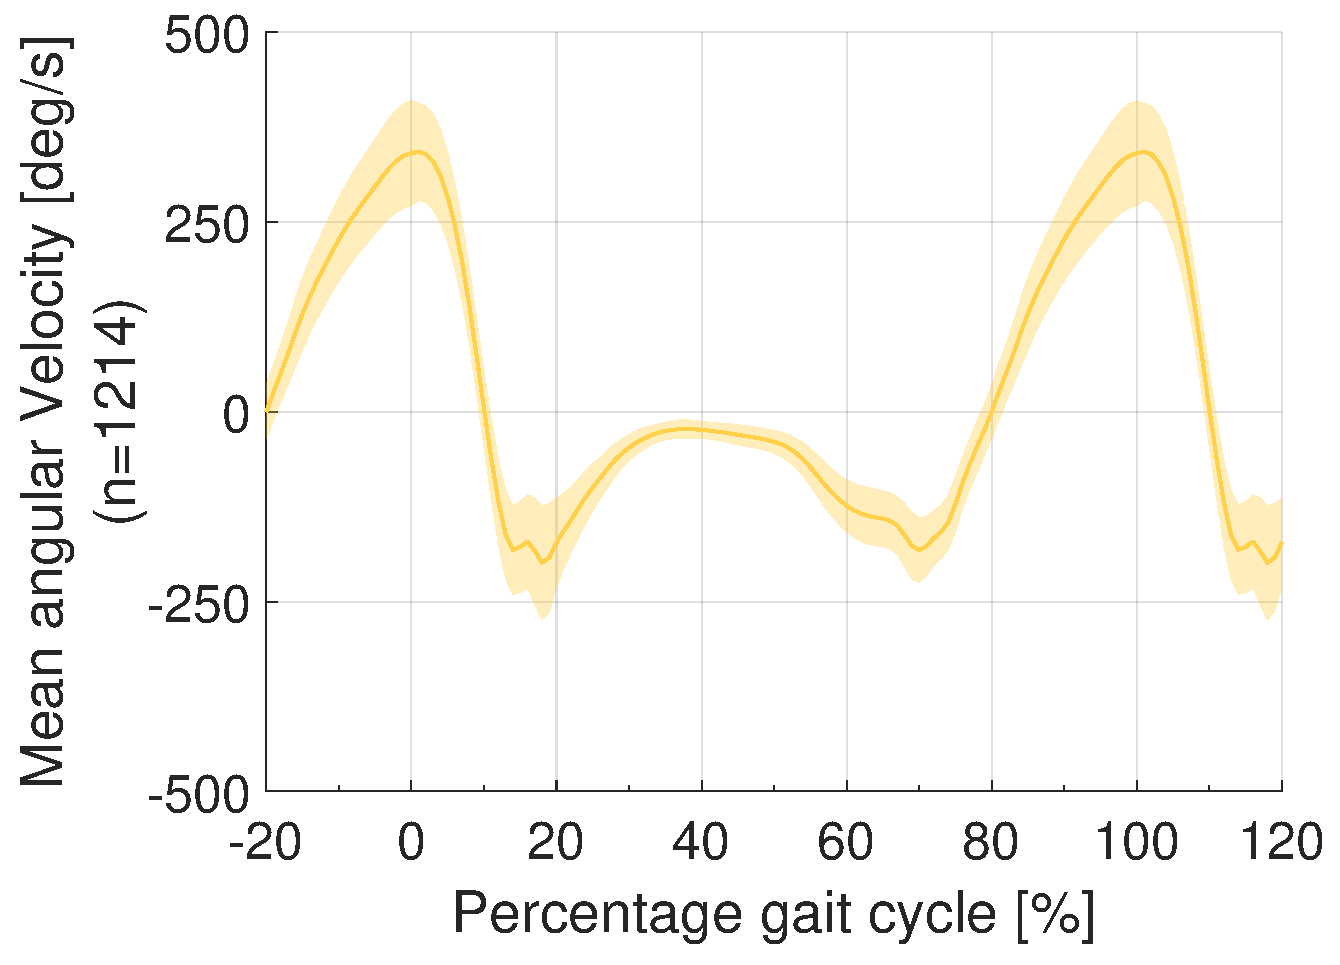
\includegraphics[width=0.275\linewidth]{content/6-Amputee/Gait-Trends/ch6_subject_01_gait_trends_r_ankle_gyro_z_activity_ramp_up.pdf} & 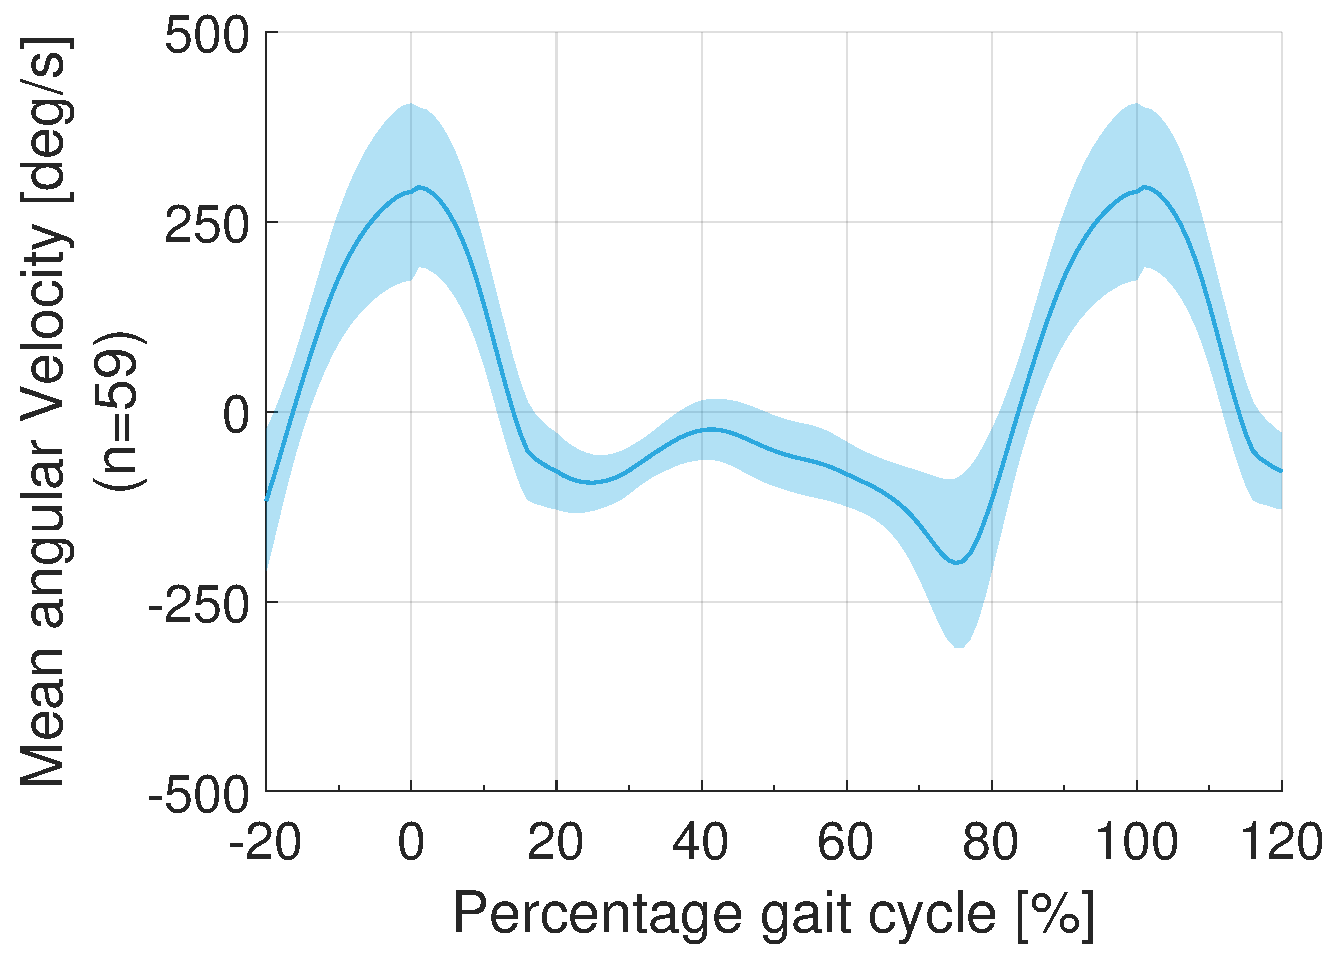
\includegraphics[width=0.275\linewidth]{content/6-Amputee/Gait-Trends/ch6_amputee_gait_trends_l_ankle_gyro_z_activity_ramp_up.pdf} &
        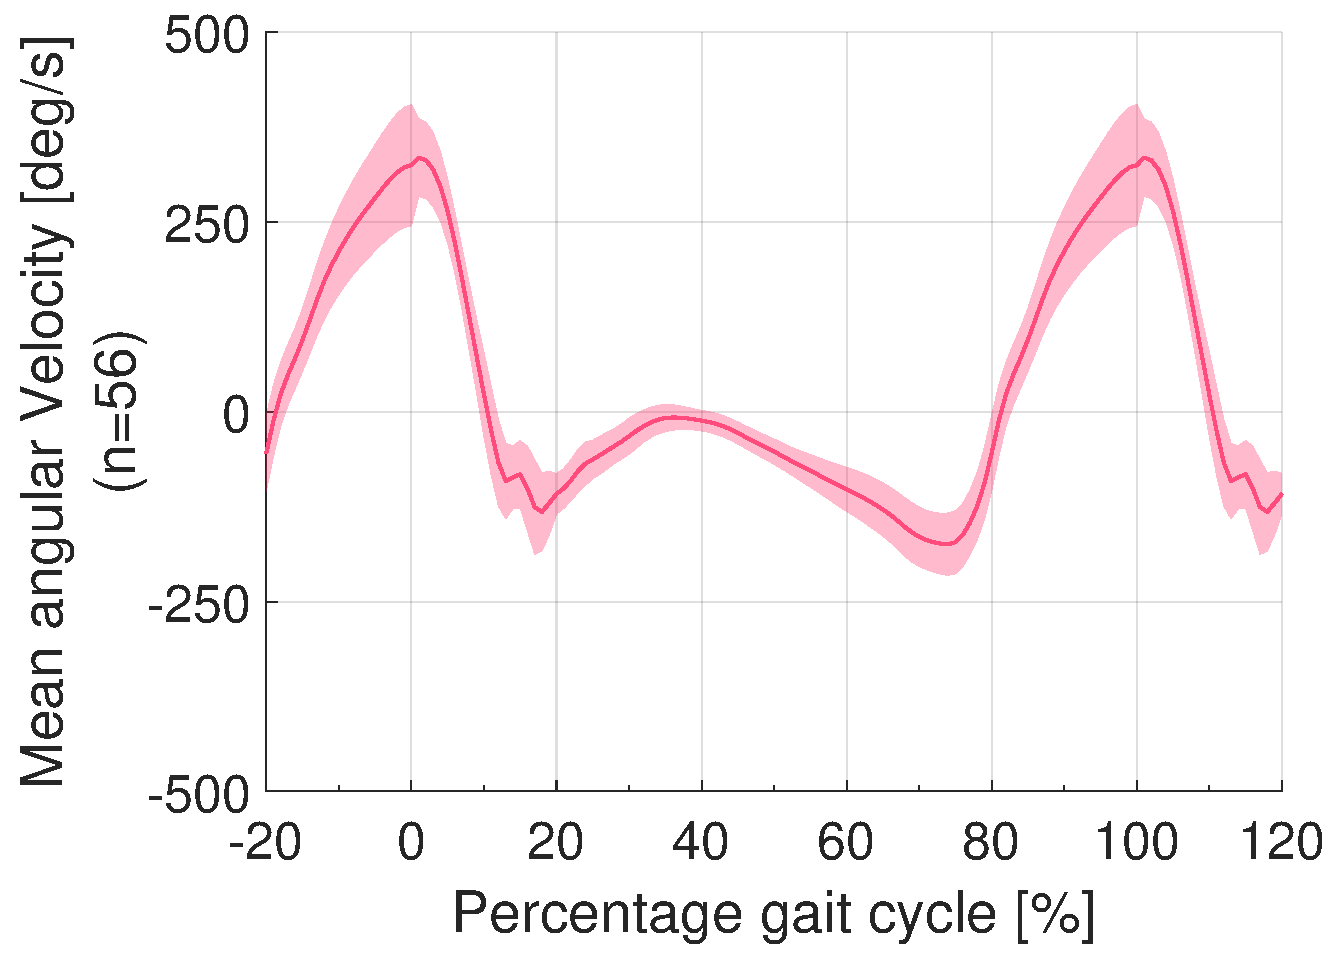
\includegraphics[width=0.275\linewidth]{content/6-Amputee/Gait-Trends/ch6_amputee_gait_trends_r_ankle_gyro_z_activity_ramp_up.pdf} \\
        
        \rotatebox{90}{\quad \textbf{Ramp Descent}} & 
        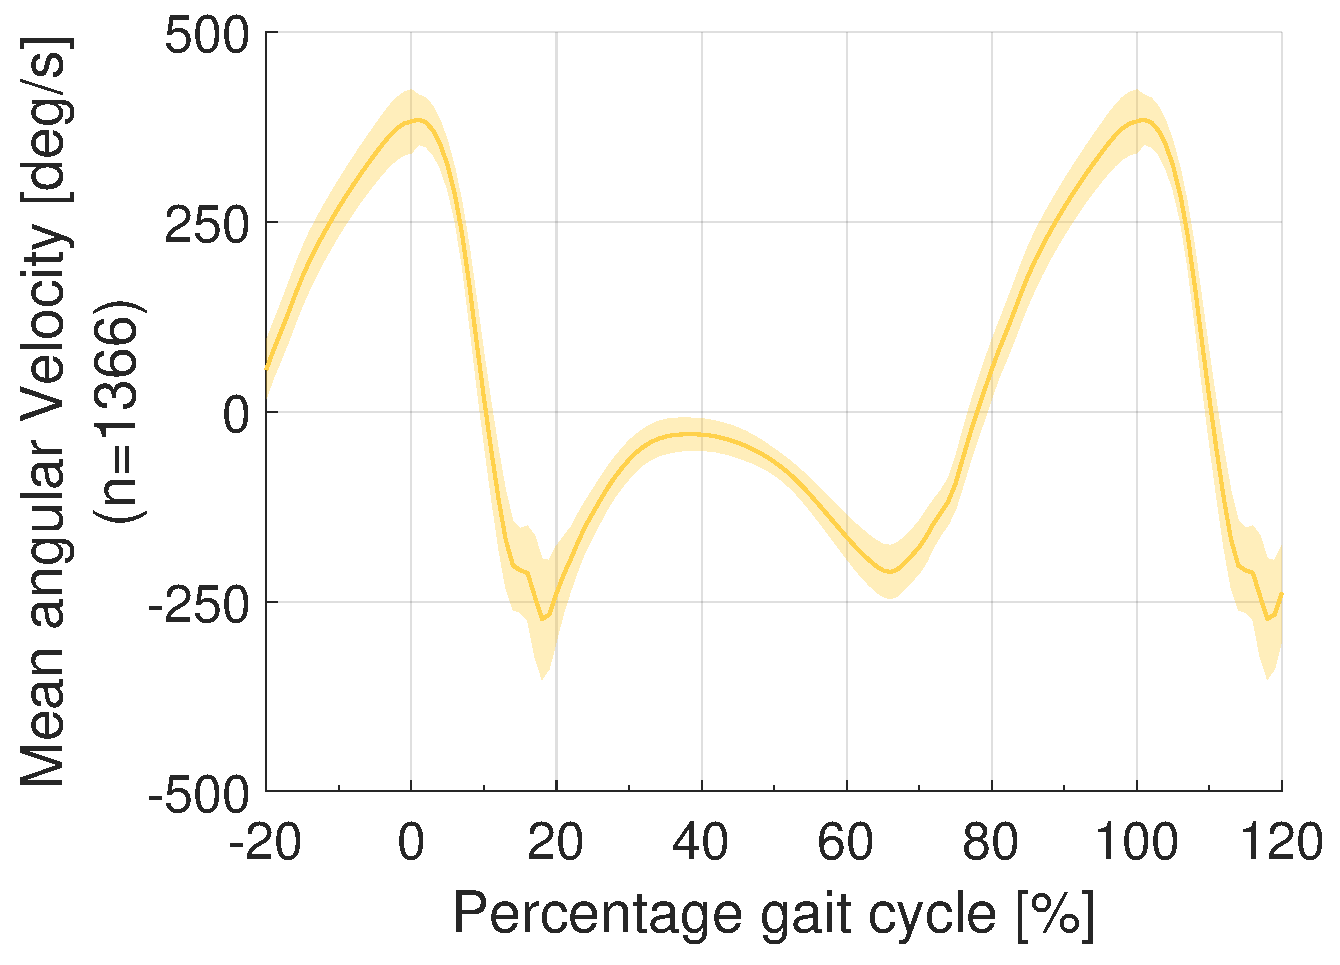
\includegraphics[width=0.275\linewidth]{content/6-Amputee/Gait-Trends/ch6_subject_01_gait_trends_r_ankle_gyro_z_activity_ramp_down.pdf} & 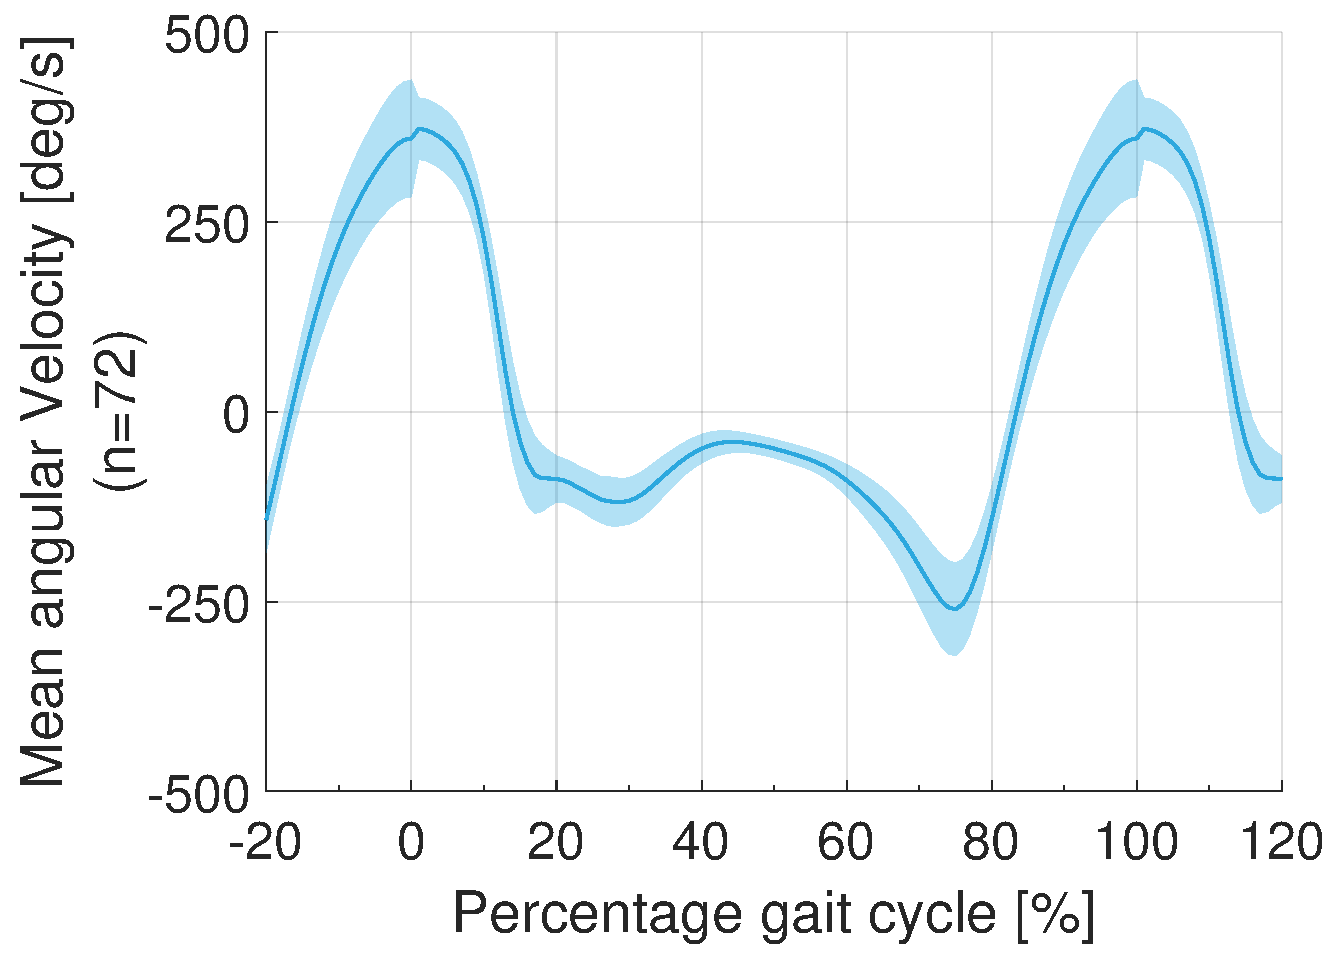
\includegraphics[width=0.275\linewidth]{content/6-Amputee/Gait-Trends/ch6_amputee_gait_trends_l_ankle_gyro_z_activity_ramp_down.pdf} &
        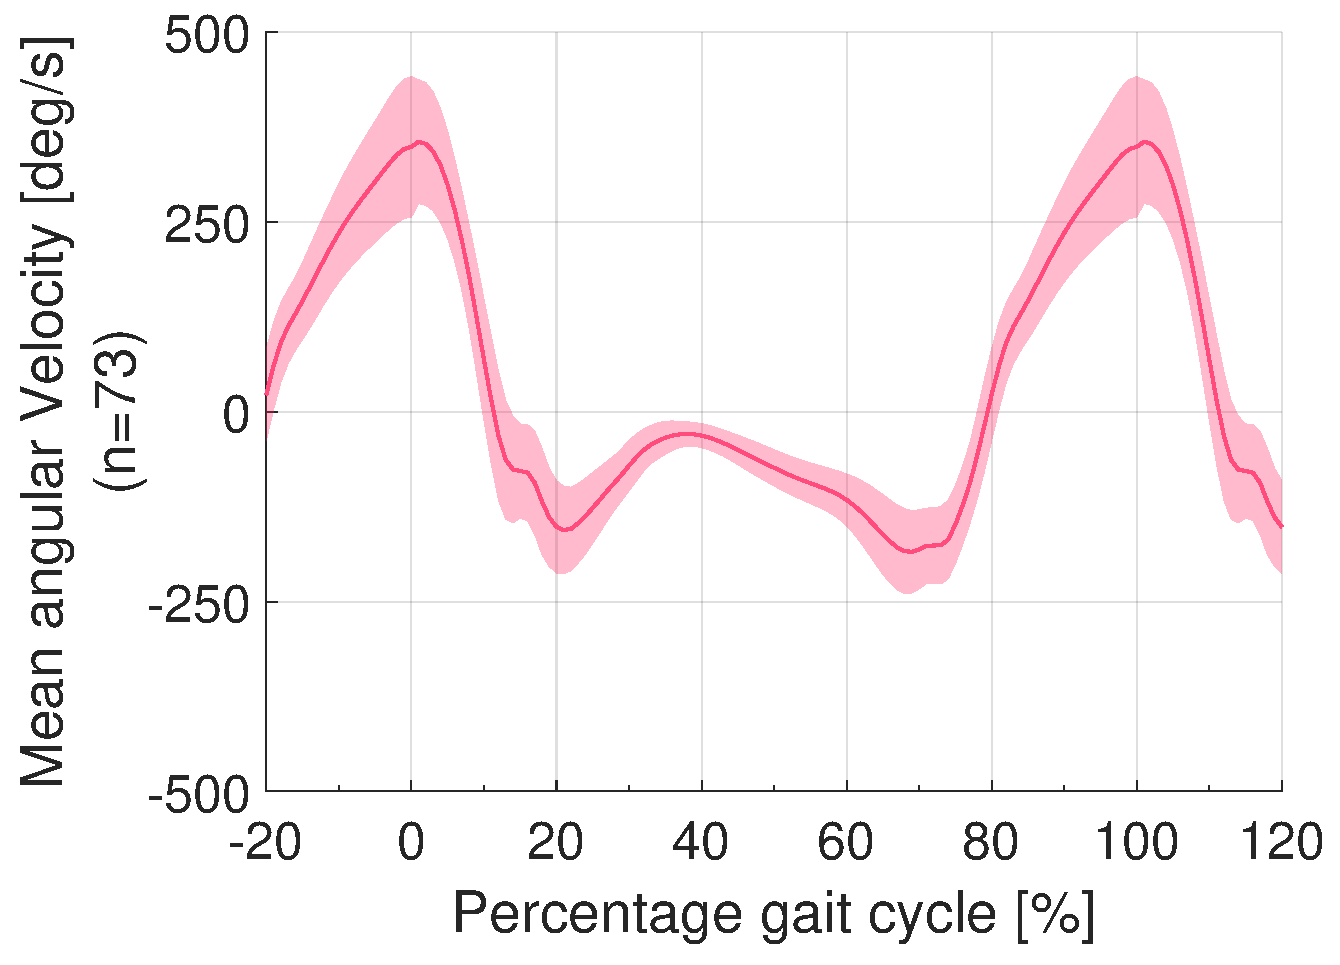
\includegraphics[width=0.275\linewidth]{content/6-Amputee/Gait-Trends/ch6_amputee_gait_trends_r_ankle_gyro_z_activity_ramp_down.pdf} \\
        
        \rotatebox{90}{~\quad \textbf{Stair Ascent}} & 
        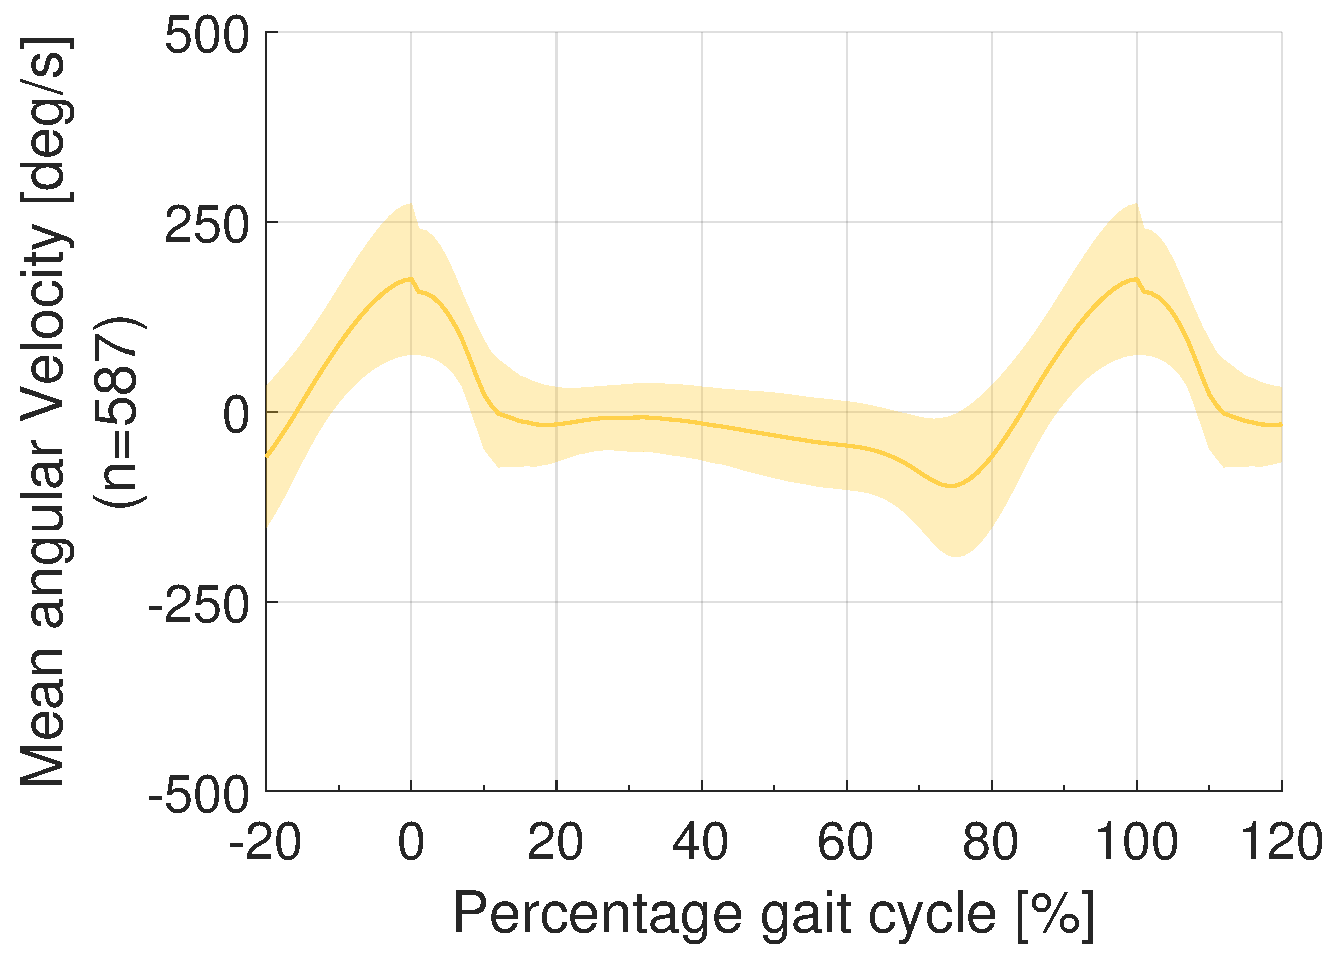
\includegraphics[width=0.275\linewidth]{content/6-Amputee/Gait-Trends/ch6_subject_01_gait_trends_r_ankle_gyro_z_activity_stair_up.pdf} & 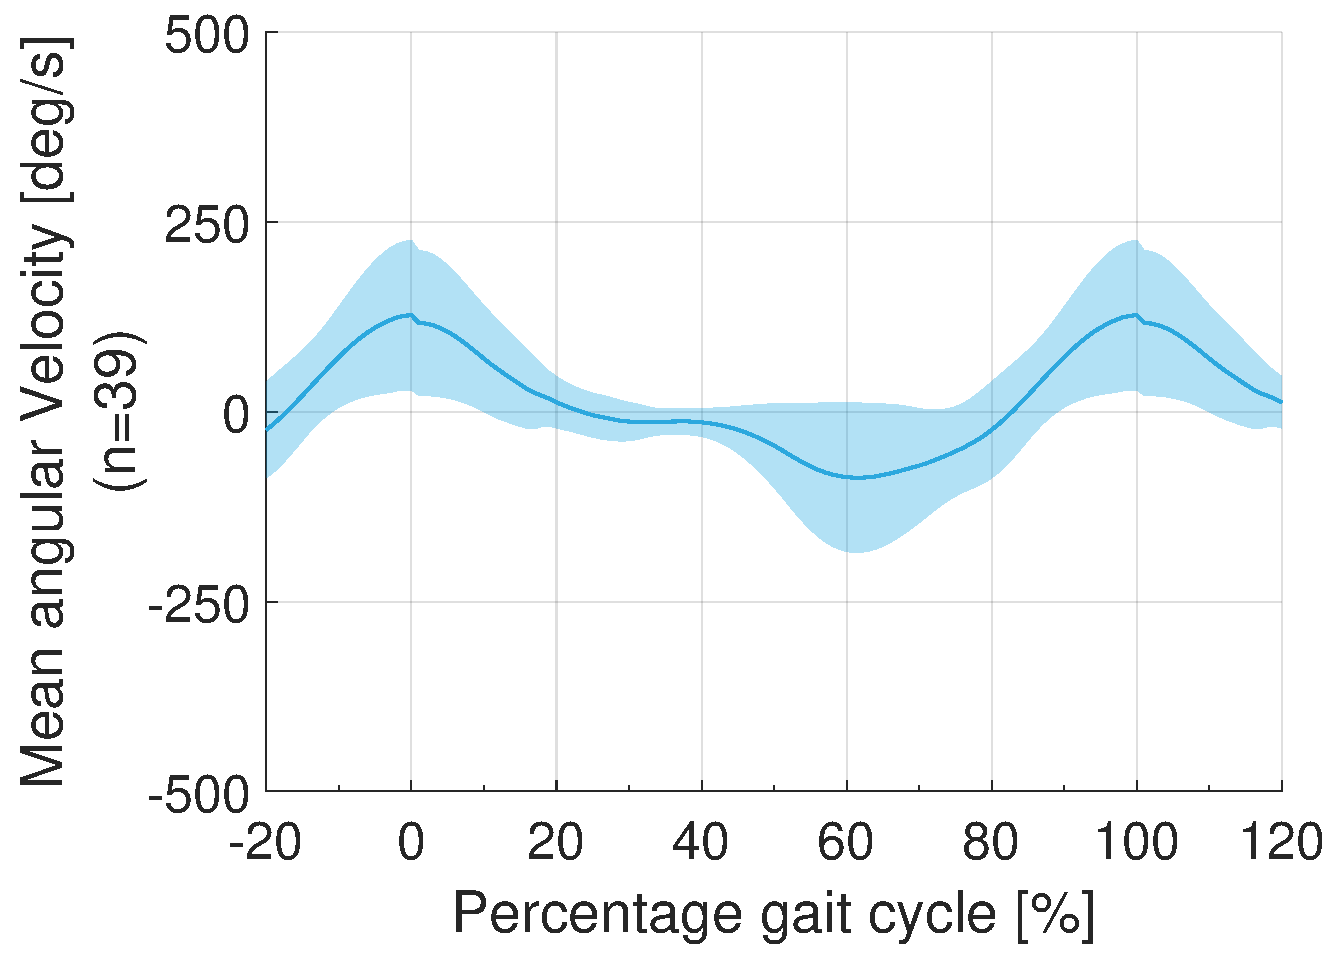
\includegraphics[width=0.275\linewidth]{content/6-Amputee/Gait-Trends/ch6_amputee_gait_trends_l_ankle_gyro_z_activity_stair_up.pdf} &
        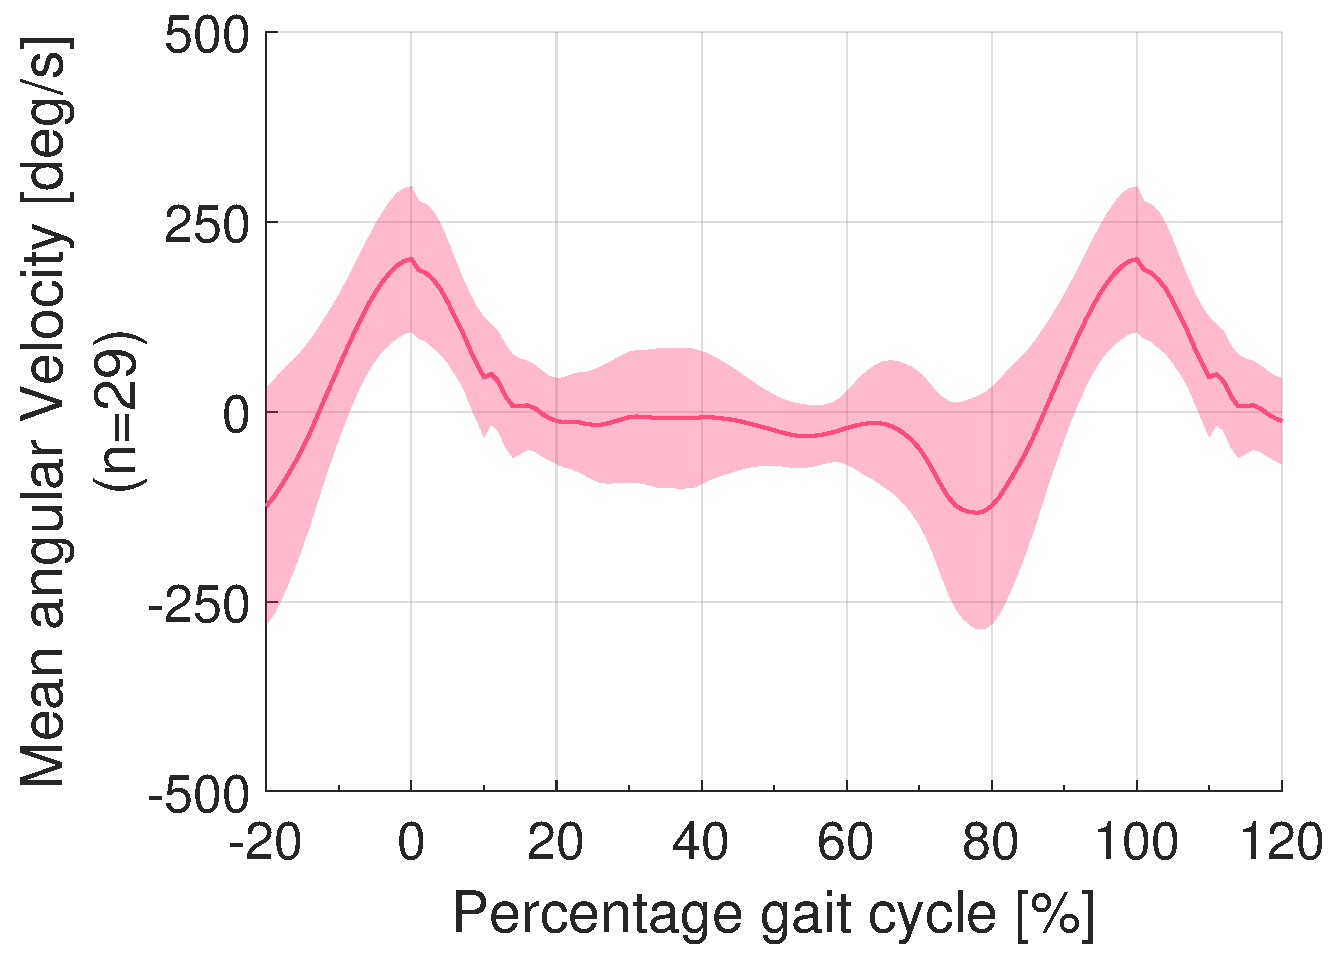
\includegraphics[width=0.275\linewidth]{content/6-Amputee/Gait-Trends/ch6_amputee_gait_trends_r_ankle_gyro_z_activity_stair_up.pdf} \\
        
        \rotatebox{90}{\quad \textbf{Stair Descent}} & 
        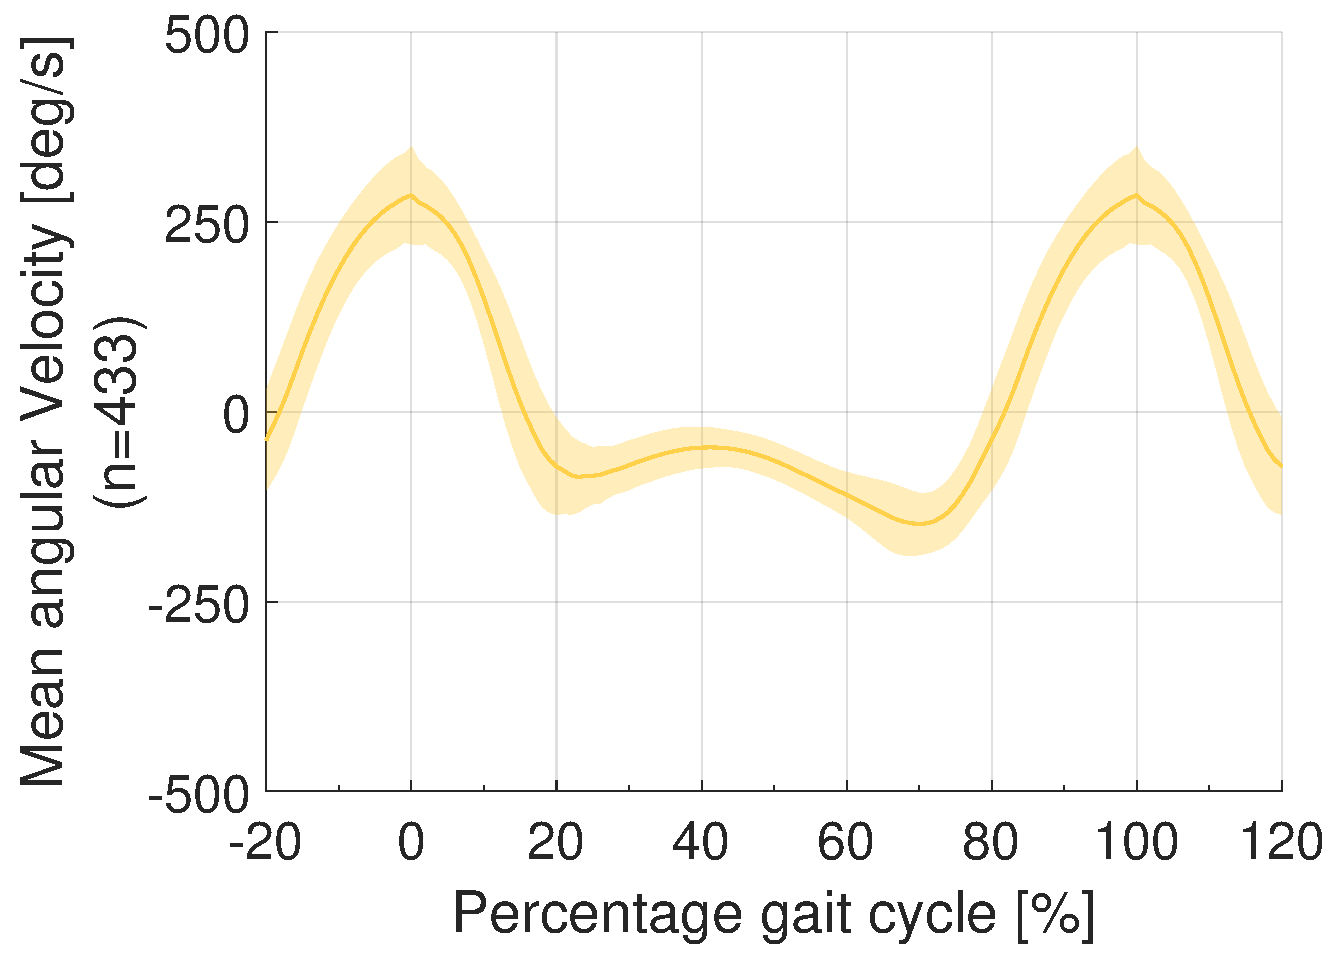
\includegraphics[width=0.275\linewidth]{content/6-Amputee/Gait-Trends/ch6_subject_01_gait_trends_r_ankle_gyro_z_activity_stair_down.pdf} & 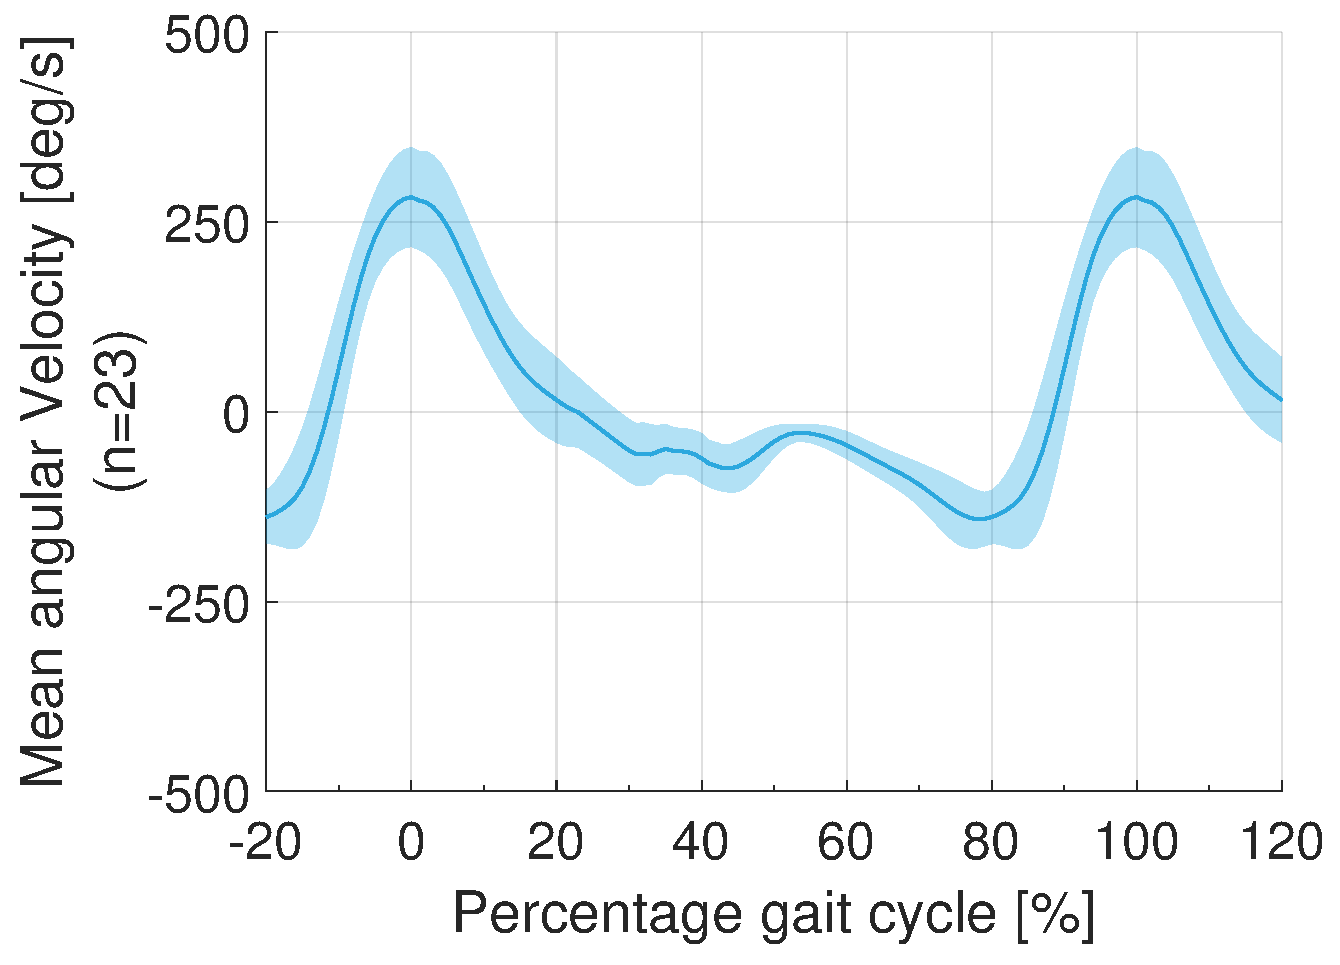
\includegraphics[width=0.275\linewidth]{content/6-Amputee/Gait-Trends/ch6_amputee_gait_trends_l_ankle_gyro_z_activity_stair_down.pdf} &
        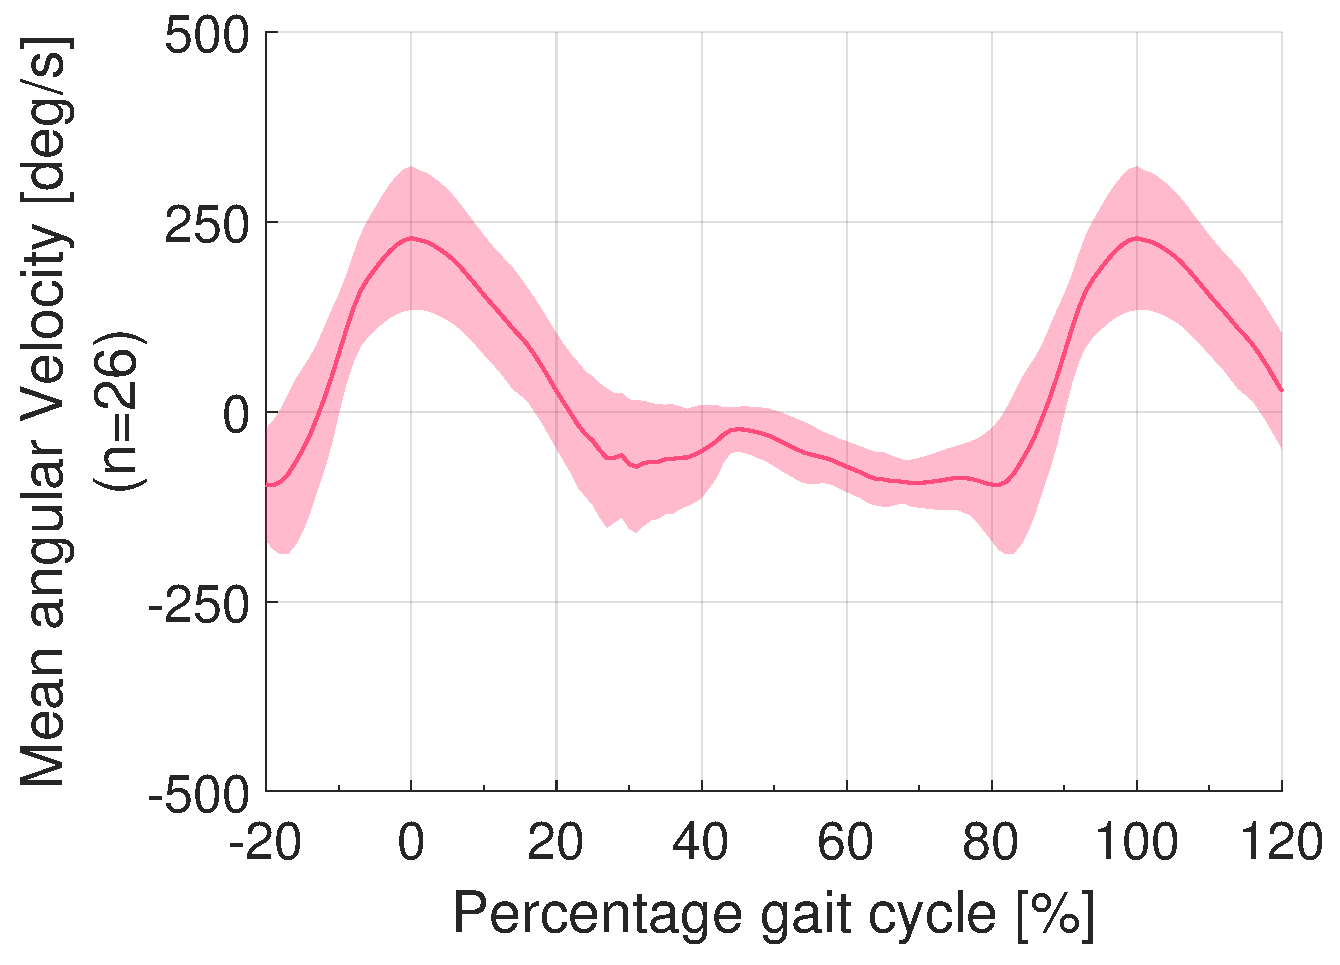
\includegraphics[width=0.275\linewidth]{content/6-Amputee/Gait-Trends/ch6_amputee_gait_trends_r_ankle_gyro_z_activity_stair_down.pdf} \\
    \end{tabular}
    \centering
    
    % \hspace*{1cm}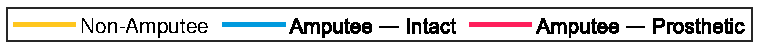
\includegraphics[width=0.7\textwidth]{content/6-Amputee/Gait-Trends/Legend.pdf}
    
    \caption[Angular velocity of the shank in the Saggital Plane during different activities for amputee and non-amputee]{Angular velocity of the shank in the Saggital Plane during different activities for amputee and non-amputee. The yellow line is for Non-Amputee (Subject 01 Left Ankle); The blue line is the intact limb of  the trans-tibial amputee; The red line is the prosthetic of the trans-tibial amputee. The solid line shows the mean of the steps recorded for each activity. The filled area represents the standard deviation.}
    \label{fig:ch6_amputee_gyro_trends}
\end{figure}


%-----------------------------------------------------------------
\section{Application of Personalisation techniques on Amputee Data}
Two techniques improved performance for non-amputees so these will be repeated here

%-----------------------------------------------------------------
\subsection{Mixed Target and Source data}

\begin{table}[hbtp]
    \caption{\hl{Classification accuracy for test data Right Ankle}}
    \label{tab:ch6-classfication-accuracy-mixed-source-target-right}
    \centering
    \begin{tabularx}{\textwidth}{cr| *{4}{Y}}
        \noalign{\hrule height 1.5pt}
        & & \multicolumn{4}{c}{\textbf{Target Training Windows}}\\
        & & 100 & 250 & 500 & 750 \\
        \hline
        \multirow{7}{*}{\rotatebox{90}{\parbox{3.4cm}{\centering\textbf{Source Training\\Windows}}}}
                 
        & 100 & $0.655{\scriptscriptstyle\pm0.06}$ & $0.711{\scriptscriptstyle\pm0.03}$ & $0.716{\scriptscriptstyle\pm0.04}$ & $0.717{\scriptscriptstyle\pm0.04}$ \\
        & 250 & $0.748{\scriptscriptstyle\pm0.01}$ & $0.693{\scriptscriptstyle\pm0.02}$ & $0.734{\scriptscriptstyle\pm0.05}$ & $0.718{\scriptscriptstyle\pm0.04}$ \\
        & 500 & $0.743{\scriptscriptstyle\pm0.03}$ & $0.653{\scriptscriptstyle\pm0.06}$ & $0.729{\scriptscriptstyle\pm0.03}$ & $\mathbf{0.751{\scriptscriptstyle\pm0.01}}$ \\
        & 750 & $0.715{\scriptscriptstyle\pm0.07}$ & $0.703{\scriptscriptstyle\pm0.07}$ & $0.693{\scriptscriptstyle\pm0.01}$ & $0.723{\scriptscriptstyle\pm0.04}$ \\
        & 1000 & $0.710{\scriptscriptstyle\pm0.04}$ & $0.744{\scriptscriptstyle\pm0.04}$ & $0.748{\scriptscriptstyle\pm0.04}$ & $0.728{\scriptscriptstyle\pm0.03}$ \\
        & 1500 & $0.723{\scriptscriptstyle\pm0.04}$ & $0.692{\scriptscriptstyle\pm0.06}$ & $0.740{\scriptscriptstyle\pm0.02}$ & $0.731{\scriptscriptstyle\pm0.04}$ \\
        & 3000 & $0.700{\scriptscriptstyle\pm0.08}$ & $0.750{\scriptscriptstyle\pm0.06}$ & $0.745{\scriptscriptstyle\pm0.08}$ & $0.733{\scriptscriptstyle\pm0.04}$ \\

        \noalign{\hrule height 1.5pt}
    \end{tabularx}
\end{table}

\begin{table}[hbtp]
    \caption{\hl{Classification accuracy for test data Left Ankle}}
    \label{tab:ch6-classfication-accuracy-mixed-source-target-left}
    \centering
    \begin{tabularx}{\textwidth}{cr| *{4}{Y}}
        \noalign{\hrule height 1.5pt}
        & & \multicolumn{4}{c}{\textbf{Target Training Windows}}\\
        & & 100 & 250 & 500 & 750 \\
        \hline
        \multirow{7}{*}{\rotatebox{90}{\parbox{3.4cm}{\centering\textbf{Source Training\\Windows}}}}
                 
        & 100 & $0.708{\scriptscriptstyle\pm0.03}$ & $0.673{\scriptscriptstyle\pm0.10}$ & $0.682{\scriptscriptstyle\pm0.01}$ & $0.715{\scriptscriptstyle\pm0.04}$ \\
        & 250 & $0.656{\scriptscriptstyle\pm0.01}$ & $0.712{\scriptscriptstyle\pm0.04}$ & $0.677{\scriptscriptstyle\pm0.05}$ & $0.721{\scriptscriptstyle\pm0.03}$ \\
        & 500 & $0.685{\scriptscriptstyle\pm0.06}$ & $0.686{\scriptscriptstyle\pm0.04}$ & $0.713{\scriptscriptstyle\pm0.04}$ & $0.736{\scriptscriptstyle\pm0.02}$ \\
        & 750 & $0.686{\scriptscriptstyle\pm0.04}$ & $0.723{\scriptscriptstyle\pm0.08}$ & $0.716{\scriptscriptstyle\pm0.04}$ & $0.696{\scriptscriptstyle\pm0.03}$ \\
        & 1000 & $0.704{\scriptscriptstyle\pm0.07}$ & $0.699{\scriptscriptstyle\pm0.03}$ & $0.730{\scriptscriptstyle\pm0.02}$ & $0.718{\scriptscriptstyle\pm0.04}$ \\
        & 1500 & $0.644{\scriptscriptstyle\pm0.04}$ & $0.705{\scriptscriptstyle\pm0.04}$ & $0.747{\scriptscriptstyle\pm0.04}$ & $0.691{\scriptscriptstyle\pm0.02}$ \\
        & 3000 & $0.730{\scriptscriptstyle\pm0.02}$ & $\mathbf{0.765{\scriptscriptstyle\pm0.04}}$ & $0.733{\scriptscriptstyle\pm0.02}$ & $0.697{\scriptscriptstyle\pm0.04}$ \\


        \noalign{\hrule height 1.5pt}
    \end{tabularx}
\end{table}


%-----------------------------------------------------------------
\subsection{Retraining a Pre-trained Model}

\begin{figure}[hbt]
    \centering
    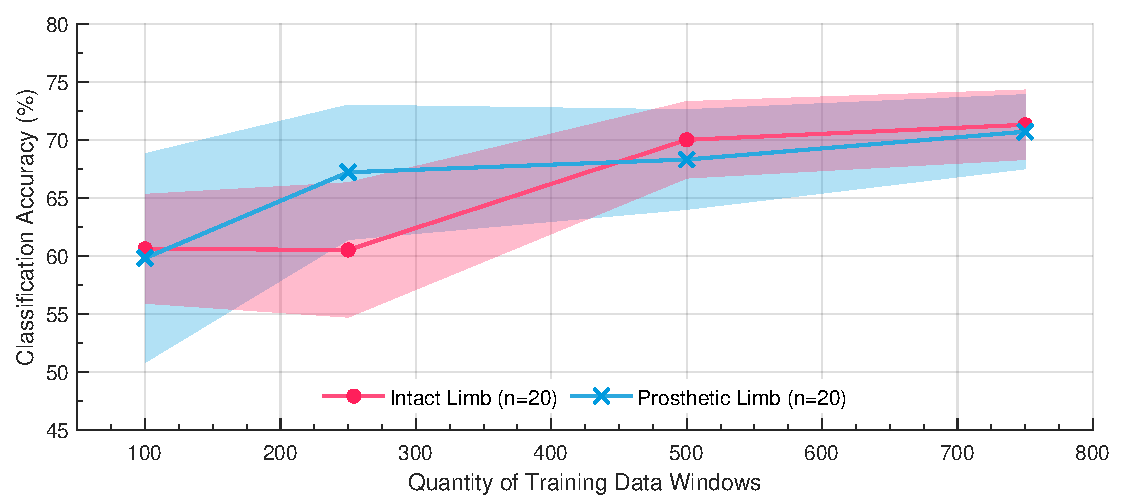
\includegraphics[width=\textwidth]{content/6-Amputee/ch6_amputee_pre_trained_model.pdf}
    \caption[Classification accuracy for re-training a pre-trained model using increasing quantities of amputee target data]{Classification accuracy for re-training a pre-trained model using increasing quantities of amputee target data. The red line shows the performance of the trained model on the intact limb of a trans-tibial amputee. The blue line shows the performance of the trained model for the prosthetic side. The filled areas represent the standard deviation. \hl{Replace image with correct data}}
    \label{fig:ch6-amputee-retrain-pre-trained}
\end{figure}


%-----------------------------------------------------------------
\section{Discussion}
What were we trying to achieve and have we achieved it?

Any interesting observations?
% Does this work act like the non-amputee?

Do any of the methods show promise?


What are the limitations of this study/methods?
%Very limited amounts of data

Areas for further work/improvements?
%Ensemble methods?
%-----------------------------------------------------------------
\section{Conclusions}
What were the research aims?

Have we met the research aims/outcomes of this work?

What are we going to do next?